\chapter{Stand der Technik}
\label{cha:Stand der Technik}

In diesem Kapitel werden alle für die Masterarbeit relevanten theoretischen Grundlagen erläutert. 
Zu erst wird in \ref{sec:Kaeltetechnik} die Thermodynamik der Kältetechnik betrachtet. 

\section{Kältetechnik}
\label{sec:Kaeltetechnik}

Die Kältetechnik wird in verschiedensten Einsatzgebieten eingesetzt, um Kälte zu erzeugen bzw. einem definierten Raum Energie in Form von Wärme zu entziehen. 

Das Konservieren von Lebensmittel ist  der ursprüngliche Hauptzwece der Kältetechnik und ist auch heute noch aktuell. Bereits 3000 Jahre v. Chr. nutzten die Ägypter und Mesopotamier Natureis, um ihre Nahrungsmittel länger haltbar zu machen.\citep{Danfoss2006}

Im Jahre 1834 meldete der US-Amerikaner Jacob Perkins sein Patent zum Thema Kältetechnik in England an. Das Patent beschreibt eine Kaltdampfmaschine in einem geschlossenen Kreislauf mit dem feuergefährlichen Äthyläther als Kältemittel.\citep{Siemens2007}

Carl von Linde baute nach konstruktiven Verbesserungen der Kaltdampfmaschine und Verwendung von Ammoniak als Kältemittel im Jahre 1876 die erste praxistaugliche Kälteanlage. Die ersten Anlagen wurden durch die Maschinenfabrik Augsburg-Nürnberg gebaut und an Brauereien sowie später auch an die Schifffahrt vertrieben.

Mit steigender Bedeutung von Elektrizität als Energieträger nach dem 1.Weltkrieg nahm auch die Entwicklung und der Bedarf an Kälteanlagen zu. Im Jahre 1920 startet die Firma General Electric mit der Serienherstellung von Haushaltkühlschränken mit Hermetik-Verdichtern.

Das vielseitige Gebiet der Kältetechnik umfasst alle Technologien, die zur Bereitstellung von Kälteenergie dienen. Sie unterscheiden sich in der benötigten zuzuführenden Energien, Einsatzbereich und eingesetzten Kältemitteln.  Zu den wichtigsten und heute meist verwendeten Technologien gehören folgende Technologien

\begin{itemize}

\item Kompressions-Kälteprozess: \textit{Prozess wird angetrieben durch Zufuhr mechanischer Energie}
\item Sorptions-Kälteprozess: \textit{Prozess wird angetrieben durch Zufuhr von Wärmeenergie}
\item Linde-Verfahren.

\end{itemize}

Weitere nicht so weitverbreitete Technologien der Kältetechnik, jedoch technisch interessante Verfahren  sind zB. das  \textit{Wirbelrohr},  \textit{Magnetische Kühlung} oder das Kühlen mittels einem Peltier-Element. Diese Verfahren werden meist nur unter hohem Energieverbrauch in Sonderfällen angewandt. \citep{Grote2014}

Da sich diese Masterarbeit mit dem Aufbau eines Prüfstandes zur Untersuchung von Abtaumethoden einer Kompressionskälteanlage beschäftigt, wird in den folgenden Kapitel ausschließlich auf diese Technologie eingegangen. Für weitere Informationen bezüglich der anderen Technologien sei an dieser Stelle auf die Literatur \citep{Baehr2013}, \citep{Grote2014} und \citep{Grote2014} verwiesen.


\subsection{Kaltdampf-Kälteprozess}
\label{subsec:Kaltdampf-Kälteprozess}

In diesem Abschnitt wird die Thermodynamik des Kaltdampf-Kälteprozesses näher erläutert. Der Kaltdampf-Kälteprozess ist ein linksläufiger \textit{Clausius-Rankine-Kreisprozess}. Die Zustandspunkte des verwendeten Kältemittels im ln p,h Diagramm sind in Abbildung \ref{fig:Schema p-h-Diagramm} dargestellt. 

\begin{figure}[htb]
\centering		
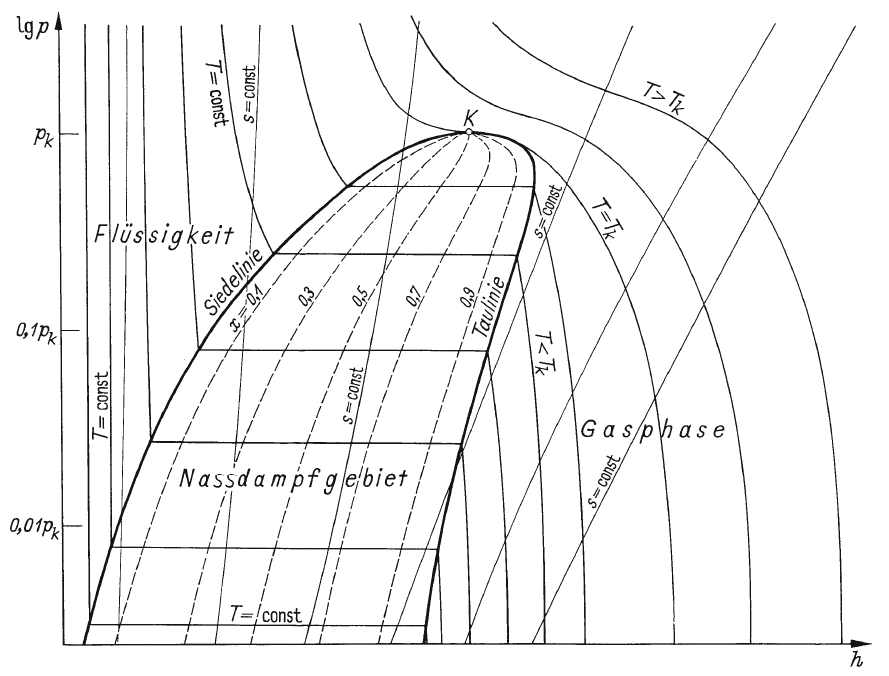
\includegraphics[width=0.75\textwidth]{Pictures/log_p_h_Beahr_Schema.png}
\caption{ln p,h-Diagramm von einem reinen Fluid  \citep{Baehr2013}}
\label{fig:Schema p-h-Diagramm}
\end{figure}

Das halb-logarithmische Diagramm ist ein vielgebrauchtes und hilfreiches Mittel in der Kältetechnik-Branche. 
\footnote{Das Zustandsdiagram wurde vom deutschen Ingenier Richard Mollier (863-1935) im Jahre 1924 erstmalig vorgestellt.} 
Im Diagramm \ref{fig:Schema p-h-Diagramm} ist der Druck logarithmisch auf der y-Achse und die spezifische Enthalpie $h$ auf der x-Achse eingetragen. Die Siedelinie ist durch $x = 0$ und die Taulinie durch $x = 1$. Zwischen $0\leqq x\leqq 1$ befindet sich das Nassdampfgebiet. Es liegt ein Gemisch aus gasförmigen und flüssigem Kältemittel vor. Der Anteil des Gases im Nassdampfgebiet wird durch $x$ ausgedrückt, $1-x$ den Anteil der Flüssigkeit.


In dem Diagramm \ref{fig:Komponeneten und p-h-Diagramm} sind alle Zustandspunkte bei einem Durchlauf des Kältekreislaufes abgebildet.Innerhalb des Nassdampfgebietes verläuft in einem idealen Kältekreislauf, eine Zustandsänderung \textit{isotherm} und \textit{isobar} ab. Wärmezu- oder abfuhr führt nicht zu einer Erhöhung der Temperatur, sondern zu einer Veränderung vom Gas- bzw. Flüssigkeitsanteil. Es wird von einer \textit{latenten}, also nicht fühlbaren,  Wärmeänderung geredet. Um einen Tropfen flüssigen Wasser, dessen Zustand sich auf der Siedelinie befindet, in einen gasförmigigen Zustand, sprich $x=1$ zu überführen, muss ihm die spezifische Verdampfungsenthalpie $\Delta h$ zugeführt werden. Verläuft die Zustandsänderung entgegengesetzt kondensiert der Tropfen und gibt die Verdampfungsenthalpie $\Delta h$ an seine Umgebung ab. 
Außerhalb des Nassdampfgebietes führt eine Wärmezu- oder abfuhr zu einer Veränderung der Temperatur. Die Wärmeänderung ist \textit{sensibel}. 

\begin{figure}[htb]
\centering		
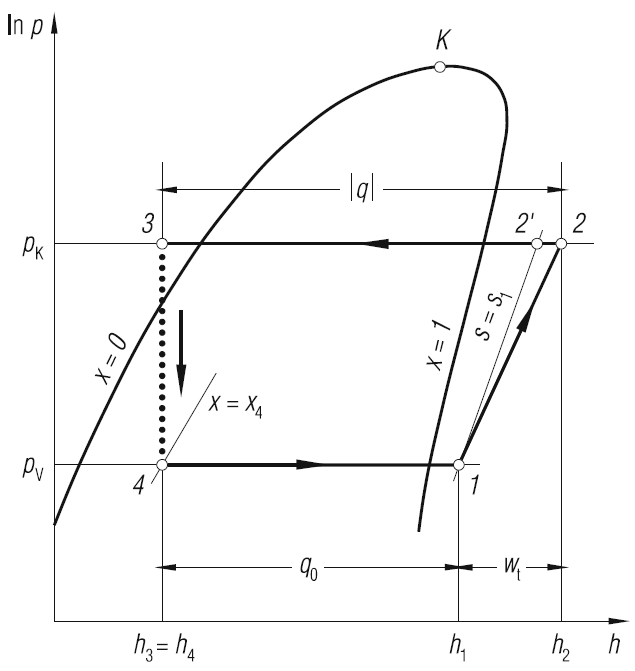
\includegraphics[width=0.6\textwidth]{Pictures/log_p_h_Beahr.png}
\caption{Kreisprozess im ln p,h-Diagramm \citep{Baehr2013}}
\label{fig:Komponeneten und p-h-Diagramm}
\end{figure}


In einem  Kaltdampfprozess, sprich ohne Verluste durch Reibung, finden folgende vier Teilprozesse statt:

\begin{itemize}
\item[1 $\longrightarrow$ 2] Kompression des dampfförmigen Kältemittels unter der Zuführung von elektrischer Leistung $P_{KM}$
\item[2 $\longrightarrow$ 3] Abkühlung, Kondensation und Unterkühlung des Kältemittels unter der Abgabe der Wärmeenergie $\dot{Q}$ über den Verflüssiger an die Umgebung
\item[3 $\longrightarrow$ 4] Entspannung des flüssigen Kältemittels durch das Drosselventil; teilweise setzt die Verdampfung des Fluids ein 
\item[4 $\longrightarrow$ 1] Verdampfung des noch flüssigen Kältemittels auf niedrigem Druckniveau unter der Aufnahme des Wärmestromes $\dot{Q_0}$ aus dem Kühlraum
\end{itemize}

Der Prozess findet auf zwei Durckniveaus statt: dem Verdampfungsdruck $p_V$ und dem Kondensationsdruck $p_K$. Die Verflüssigung des Kältemittels findet auf hohem Druckniveau und die Verdampfung auf niedrigem Druck statt. Die höchste Temperatur wird nach der Kompression am Zustandspunkt 2 erreicht; er befindet sich im Überhitzen- und Hochdruckbereich. Die niedrigste Temperatur ist kurz nach dem Dosselventil und vor dem Verdampfer am Punkt 4. auf niedrigem Druckniveau. 

Nach dem Anwenden des 1. Hauptsatzes der Thermodynamik, die Erhaltung der Energie in einem System, auf den Kältekreislauf folgt die Gleichung :

 \begin{equation}
 	|\dot{Q}|  = \dot{Q_0} +  P_{KM}.
 	\label{eq:Energiebilanz}
 \end{equation}
 
Die elektrische Antriebsleistung der Kältemaschine ist die aufgenommene elektrische Leistung durch den Kompressor zwischen den Zustandspunkten 1  und 2. Sie ergibt sich zu:

\begin{equation}
P_{KM} = \dot{m}~ w_t= \dot{m}~ (h_2 - h_1) = \frac{\dot{m} }{\eta_{sV}} (h_{2'}- h_1).
\label{eq:Antriebsleistung}
\end{equation}

Hierbei ist $\eta_{sV}$ der isentrope Wirkungsgrad des Kompressors. Der isentrope Wirkungsgrad setzt den realen Kältekreislauf in ein Verhältnis zum idealen Kältekreislauf. Die Überhitzung des Gases am Austritt des Kompressors ist höher als die Überhitzung nach einer isentropen Verdichtung. Daraus folgt eine höhere Energieaufnahme durch den Kompressor und ein höherer Wärmestrom $\dot{Q}$, der über den Verflüssiger an die Umgebung abgegeben werden muss. Der isentrope Wirkungsgrad ist definiert über 

\begin{equation}
\eta_{sV}:= \frac{h_{2'}- h_{1}}{h_2 - h_1}.
\label{eq:Antriebsleistung}
\end{equation}


Der Wärmestrom $\dot{Q}$ wird über den Verflüssiger zwischen den Zuständen 2 und 3 abgeführt. Die Formel von  $\dot{Q}$ lautet: 

\begin{equation}
	\dot{Q} = \dot{m}~q_0 = \dot{m}~ (h_3 - h_2)< 0.
	\label{eq:Wärmestrom}
\end{equation}

Der Wärmestrom $\dot{Q}$ ist immer kleiner als Null; er wird dem Kreislauf folglich entzogen.  
 
Über ein Drosselorgan wird das Kältemittel vom hohen Druckniveau auf das niedrigere Druckniveau entspannt. Der Teilprozess findet zwischen den Zustandspunkten 3 und 4 statt und wird als $isenthalp$ angenommen.  
 
Die Kälteleistung $\dot{Q_0}$, sprich den aus dem Kühlraum zu entnehmender Wärmestrom, ergibt sich aus dem Kältemittel-Massenstrom $\dot{m}$ und den spezifischen Enthalpien der Zustände 4 und 1 :

\begin{equation}
	\dot{Q_0} = \dot{m}~ q_0 = \dot{m}~ (h_1 - h_4).
	\label{eq:Kälteleistung}
\end{equation}




Die Bewertung einer Kälteanlage erfolgt durch die Leistungszahl $\epsilon_{KM}$: 

\begin{equation}
	\epsilon_{KM} := \frac{Kälteleistung}{Antriebsleistung} =\frac{\dot{Q_0}}{P_{KM}}.
	\label{eq:Leistungszahl}
\end{equation}

Ziel bei der Auslegung und dem Betrieb einer Kältemaschine ist eine möglichst große Leistungszahl zu erlangen. Damit $\epsilon_{KM}$ groß wird, muss die Kälteleistung $\dot{Q_0}$ groß werden und die aufgewandte Verdichterleistung $P_{KM}$ klein werden. 
%\subsection{•}
%\label{•}

\subsection{Komponenten eines Kaltdampfprozesses}
\label{subsec:Komponenten eines Kaltdampfprozesses}

Die Komponenten für einen einfachen Kaltdampfprozess  besteht aus vier Komponenten:

\begin{itemize}
\item der Kompressor
\item der Verflüssiger 
\item das Drosselvenil Expansionsventil
\item der Verdampfer. 
\end{itemize}

In Abbildung \ref{fig:einfacher Kältekreislauf} sind die vier Komponenten mit ihren Zustandspunkten dargestellt.

Der Kompressor bildet das Herzstück der Kälteanlage. Er verdichtet das gasförmige Kältemittel von niedrigem Druck auf ein höheres Druckniveau. Um diese Arbeit zu verrichten, wird der Verdichter mit elektrischer Energie versorgt. Der Kompressor gibt es in verschiedenen Bauvarianten. Die zwei wichtigsten Bauvarianten sind der \textit{Hubkolbenverdichter} und der \textit{Rotationskolbenverdichter}. Die Baugruppen der Verdichter werden in offene, halbhermetische und vollhermetische Verdichter unterschieden.  Schrauben-,Scroll- sowie Turboverdichter sind Bauarten der \textit{Rotationskolbenverdichter}. 

\begin{figure}[htb]
\centering		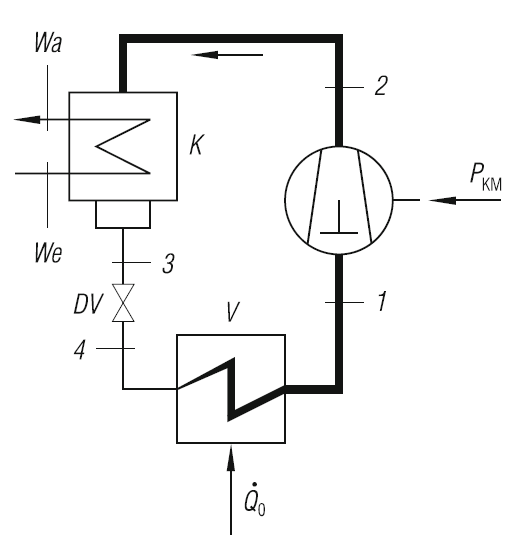
\includegraphics[width=0.50\textwidth]{Pictures/Kaltekreislauf_beahr.png}
\caption{Einfacher Kältekreislauf}
\label{fig:einfacher Kältekreislauf}
\end{figure}


